\chapter{Surface (Triangle mesh)}
\label{cap_surface}

At InVesalius, a 3D surface is generated based on a image segmentation. A surface is generated using the \textit{marching cubes} algorithm. In a nutshell, this algorithm transforms \textit{voxels} from the stacked and segmented images to polygons (triangles in this case).

On the left panel, inside \textbf{3. Configure 3D surface}, \textbf{Surface properties} you have the controls to configure a 3D surface.

\begin{figure}[!htb]
\centering
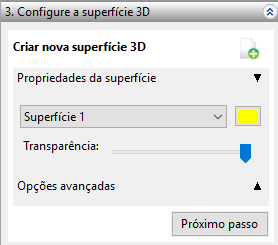
\includegraphics[scale=0.65]{surface_config_panel_pt.png}
\caption{3D surface configuration.}
\label{fig:3d_surface_managment}
\end{figure}


\section{Creating 3D surfaces}

It's possible create a new surface based on a already segmented mask. To do that, on the left panel, \textbf{3. Configure 3D surface}, click on the button shown at the figure~\ref{fig:shortcut_new_surface}.

\begin{figure}[!htb]
\centering

\includegraphics[scale=0.18]{object_add_original}
\caption{Button to create a 3D surface.}
\label{fig:shortcut_new_surface}
\end{figure}

After clicking this button a dialog will be shown (figure \ref{fig:create_surface_1}). This dialog allows to configure the 3D surface creation. It allows to set the quality of the surface, to fill the surface holes and to keep only the largest connected region of the surface.

\begin{figure}[!htb]
\centering
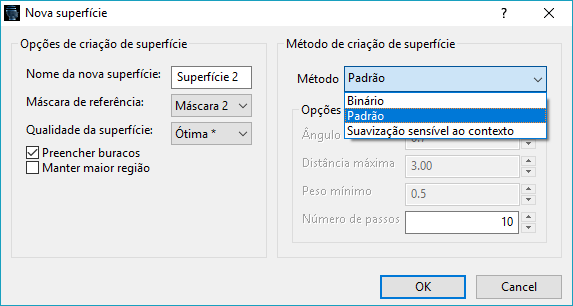
\includegraphics[scale=0.5]{surface_config_window_pt.png}
\caption{3D surface creation dialog.}
\label{fig:create_surface_1}
\end{figure}

%Existe 2 opções para fechar os buracos existentes e para selecionar a maior região da superfície aonde em muitos
%casos é útil para remover o suporte ou a mesa do tomografo.

The keep largest region option may be used, for instance, to remove the tomograph support. Figure~\ref{fig:surface_ex1} displays a surface created with \textbf{Keep largest region} and \textbf{Fill holes} activated. 

\begin{figure}[!htb]
  \centering
  \subfloat[Frente]{\label{fig:__1}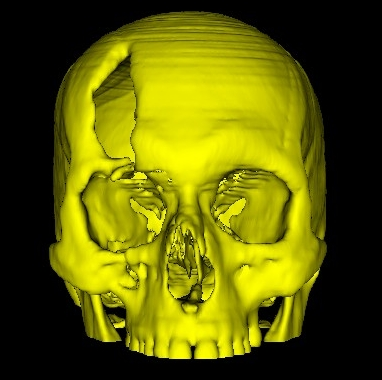
\includegraphics[width=0.338\textwidth]{surface_model_front.jpg}}
  \subfloat[Baixo]{\label{fig:__1}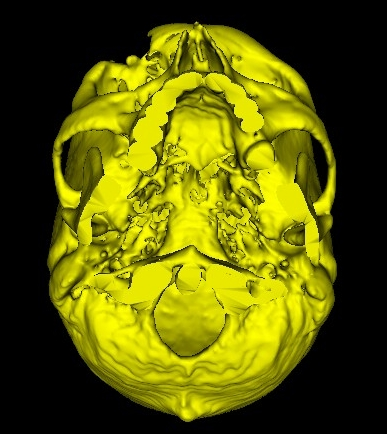
\includegraphics[width=0.3\textwidth]{surface_model_bottom.jpg}}
  \caption{Surface created with the options \textbf{Keep largest region} and \textbf{Fill holes} activated.}
  \label{fig:surface_ex1}
\end{figure}

Whereas the figure~\ref{fig:surface_ex2} displays the surface create without activating that options. Note the tomograph support and the holes.

\begin{figure}
  \centering
  \subfloat[Frente]{\label{fig:__2}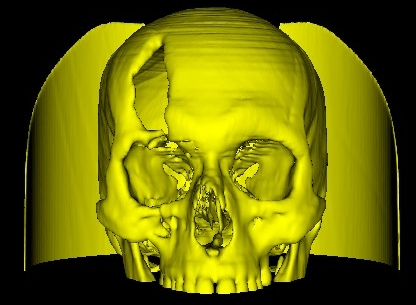
\includegraphics[width=0.371\textwidth]{surface_model_front_all_parts.jpg}}
  \subfloat[Baixo]{\label{fig:__2}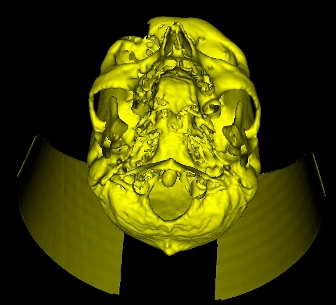
\includegraphics[width=0.3\textwidth]{surface_model_bottom_all_parts.jpg}}
  \caption{Surface created with the options \textbf{Keep largest region} and \textbf{Fill holes} deactivated.}
  \label{fig:surface_ex2}
\end{figure}

The item \textbf{Surface creation method} has the following options:\textbf{Binary}, \textbf{Context aware smoothing} and \textbf{Default}. Figure~\ref{fig:surf_method} shows an example of surface created using each of these 3 methods.

The \textbf{Binary} method takes as input the segmentation mask which is binary, where selected regions have value 1 and non-selected have value 0. As it is binary, the surface generated has a blocky aspect, mainly in high curvature areas, appearing staircases.

\textbf{Context aware smoothing} starts generating the surface using binary method. After that it uses the algorithm \textbf{Context aware smoothing} to smooth the surface to avoid the staircase artifacts. This method has 4 parameters presented bellow.

The \textbf{angle} parameter is the angle between 2 adjacent triangles. If the calculated angle is \textbf{greater than} the angle parameter the triangle will be considered a staircase triangle and will be smoothed. The angle parameter ranges from $0$ to $1$. Where $0$ is $0^\circ$  and $1$ is $90^\circ$. The \textbf{Max distance} is the maximum distance that a non-staircase triangle has to be from a staircase triangle to be considered to be smoothed. Non-staircase triangles with distance greater than \textbf{Max distance} also will be smoothed but the smoothing will be weighted by the \textbf{Min. weight} parameter. This parameter ranges from $0$ (without smoothing) to $1$ (total smoothing). The last parameter, \textbf{N. steps}, is the number of times the smoothing algorithm will be run. The greater this parameter the smoother the surface will be.

The \textbf{Default} method is enable only when \textbf{it was used thresholding segmentation and there is not a manual edition in the mask}. This method doesn't use the mask image, but the exam image, and generates a smoother surface.

\begin{figure}[!htb]
  \centering
  \subfloat[Binary]{\label{fig:surf_binary}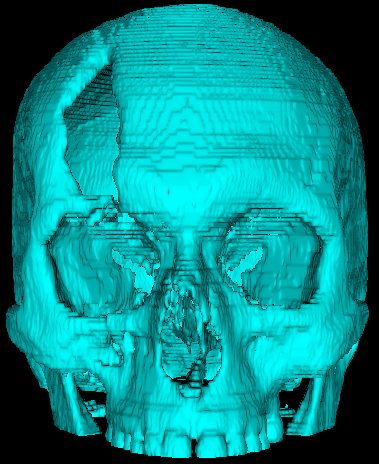
\includegraphics[width=0.33\textwidth]{binary.png}}
  \hfill
  \subfloat[Context aware]{\label{fig:surf_context}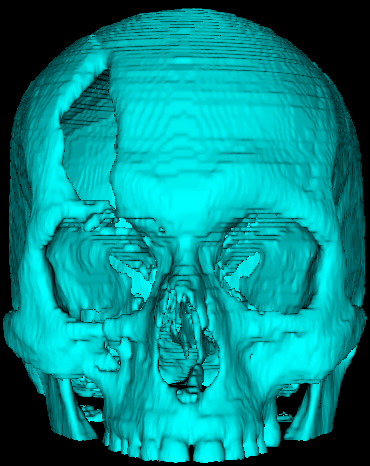
\includegraphics[width=0.32\textwidth]{context.png}}
  \hfill
  \subfloat[Default]{\label{fig:surfa_default}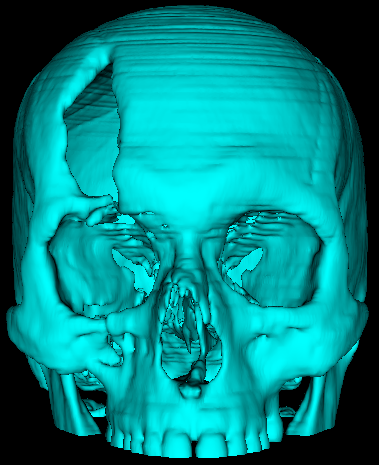
\includegraphics[width=0.332\textwidth]{default.png}}
  \caption{Surface generated by each method.}
  \label{fig:surf_method}
\end{figure}

\section{Transparency}

It's also possible to display a surface with some level of Transparency. To do that, first select the desired surface from the list of surfaces, in the item \textbf{3. Configure 3D surface}, \textbf{Surface properties} (figure \ref{fig:select_surface}).

\begin{figure}[!htb]
\centering
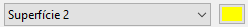
\includegraphics[scale=0.8]{surface_select_menu.png}
\caption{Surface selection.}
\label{fig:select_surface}
\end{figure}

Then, to set the level of surface transparency, use de sliding control shown in the figure~\ref{fig:select_transparency}. The more to right the more transparent the surface will be shown.

\begin{figure}[!htb]
\centering
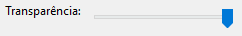
\includegraphics[scale=0.7]{surface_transparency_pt.png}
\caption{Selection of surface transparency.}
\label{fig:select_transparency}
\end{figure}

Figure~\ref{fig:model_transparency} shows 2 surfaces: the extern surface (green color) has some level of transparency which permits to see the intern surface (yellow color).

\begin{figure}[!htb]
\centering
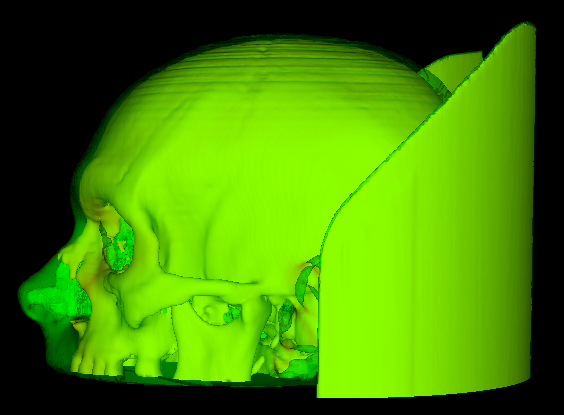
\includegraphics[scale=0.3]{transparency_2}
\caption{Surface with transparency.}
\label{fig:model_transparency}
\end{figure}

\newpage

\section{Color}

It's possible to change a surface color. Select the surface (see figure~\ref{fig:select_surface}). Click on the colored button on the right to the surface selection list. Figure~\ref{fig:change_surface_color} displays this button, inside the item \textbf{3. Configure 3D surface}, \textbf{Surface properties}.

\begin{figure}[!htb]
\centering
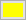
\includegraphics[scale=0.6]{surface_button_select_color_yellow.png}
\caption{Button to change surface color.}
\label{fig:change_surface_color}
\end{figure}

A dialog will be shown (figure~\ref{fig:button_select_color}). Select the desired color and click on \textbf{Ok}.

\begin{figure}[!htb]
\centering
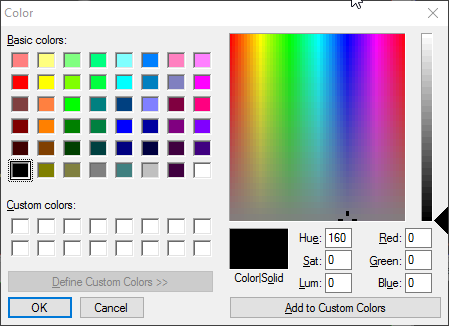
\includegraphics[scale=0.6]{surface_select_color_windows_so_en.png}
\caption{Color dialog.}
\label{fig:button_select_color}
\end{figure}

\section{Splitting disconnected surfaces}

To split disconnected surfaces it's necessary to go to \textbf{3. Configure 3D surface}, \textbf{Advanced options} (figure~\ref{fig:advanced_tools}).

\begin{figure}[!htb]
\centering
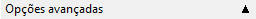
\includegraphics[scale=0.7]{surface_painel_advanced_options_pt.png}
\caption{Advanced options.}
\label{fig:advanced_tools}
\end{figure}

\newpage

The advanced options panel will be displayed (figure~\ref{fig:advanced_tools_expanded}).

\begin{figure}[!htb]
\centering
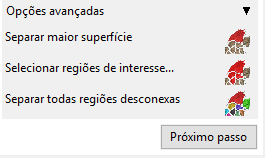
\includegraphics[scale=0.7]{surface_split_pt.png}
\caption{Advanced options panel.}
\label{fig:advanced_tools_expanded}
\end{figure}

\subsection{Select largest surface}

The option \textbf{Select largest surface} selects, automatically, only surface with the greater volume. To do this operation click on the button illustrated in the figure~\ref{fig:short_connectivity_largest}. This operation creates new surface with only the largest surface.

\begin{figure}[!htb]
\centering
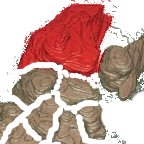
\includegraphics[scale=0.2]{connectivity_largest}
\caption{Button to split the largest disconnected surface}
\label{fig:short_connectivity_largest}
\end{figure}

As an example, the figure~\ref{fig:extract_most_region_1} shows a surface before \textbf{Select largest surface}.

\begin{figure}[!htb]
\centering
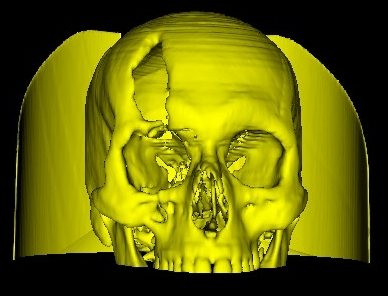
\includegraphics[scale=0.3]{surface_extract_most_region_1.jpg}
\caption{Disconnected surfaces.}
\label{fig:extract_most_region_1}
\end{figure}

Whereas the figure~\ref{fig:extract_most_region2} shows the surface with largest disconnected region separated.

\begin{figure}[!htb]
\centering
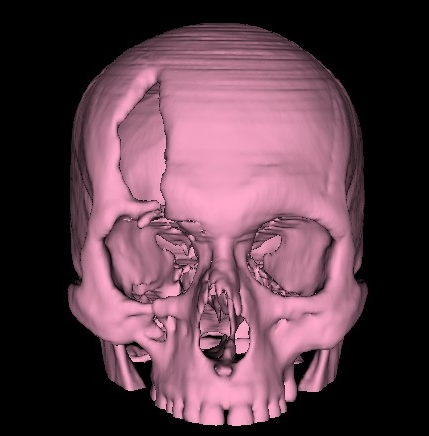
\includegraphics[scale=0.3]{surface_extract_most_region2.jpg}
\caption{Largest disconnected region separated.}
\label{fig:extract_most_region2}
\end{figure}

\newpage

\subsection{Select regions of interest}

Other selection option is \textbf{Select regions of interest ...}. To do this operation click on the button illustrated on the figure~\ref{fig:short_connectivity_manual}. Then click on desired disconnected surface regions you want to select. Next click on \textbf{Select regions of interest ...}. This operation will create new surface with only the selected disconnected regions.

\begin{figure}[!htb]
\centering
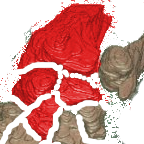
\includegraphics[scale=0.2]{connectivity_manual}
\caption{Button to select the regions of interest.}
\label{fig:short_connectivity_manual}
\end{figure}

As an example, the figure~\ref{fig:extract_most_region3} shows the surface created after the user selects the cranium and the right part of the tomograph support.

\begin{figure}[!htb]
\centering
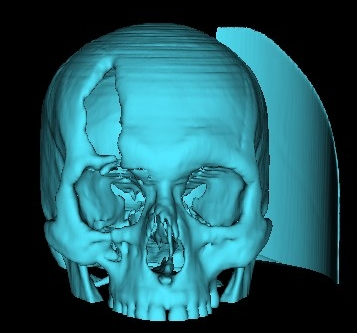
\includegraphics[scale=0.35]{surface_extract_most_region3.jpg}
\caption{Example of selected regions of interest}
\label{fig:extract_most_region3}
\end{figure}


\subsection{Split all disconnected surfaces}

It's also possible to split all the disconnected surface regions automatically. To do this, click on the button illustrated in the figure~\ref{fig:connectivity_split_all}.

\begin{figure}[!htb]
\centering
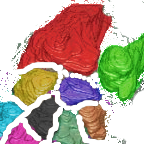
\includegraphics[scale=0.2]{connectivity_split_all}
\caption{Button to split all the disconnected regions surface.}
\label{fig:connectivity_split_all}
\end{figure}

Figure~\ref{fig:extrac_most_region_4} shows an example.

\begin{figure}[!htb]
\centering
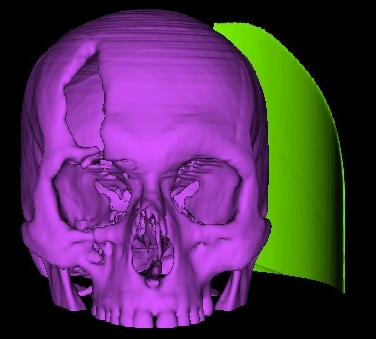
\includegraphics[scale=0.3]{surface_extract_most_region_4.jpg}
\caption{Example of split all disconnected regions surface.}
\label{fig:extrac_most_region_4}
\end{figure}

